% This is samplepaper.tex, a sample chapter demonstrating the
% LLNCS macro package for Springer Computer Science proceedings;
% Version 2.20 of 2017/10/04
%
\documentclass[runningheads]{llncs}
\setcounter{secnumdepth}{5}
%
\usepackage{graphicx}
% Used for displaying a sample figure. If possible, figure files should
% be included in EPS format.
%
% If you use the hyperref package, please uncomment the following line
% to display URLs in blue roman font according to Springer's eBook style:
% \renewcommand\UrlFont{\color{blue}\rmfamily}

\usepackage{todonotes}
\usepackage{xcolor}
\usepackage{listings}
\usepackage{mdframed}
\usepackage{caption}
%\usepackage{todo}

\usepackage{array}
\newcolumntype{H}{>{\setbox0=\hbox\bgroup}c<{\egroup}@{}}

\begin{document}
%
\title{Saving Energy Using the READEX Methodology \thanks{The research leading to these results has received funding from the European Union's Horizon 2020 Programme under grant agreement number 671657.}}
%
%\titlerunning{Abbreviated paper title}
% If the paper title is too long for the running head, you can set
% an abbreviated paper title here
%
\author{Madhura Kumaraswamy \inst{1} \and Anamika Chowdhury \inst{1} \and Michael Gerndt \inst{1} \and
Nico Reissmann \inst{2} \and Per Gunnar Kjeldsberg \inst{2} \and
Ondrej Vysocky \inst{3} \and Jan Zapletal \inst{3} \and Lubomir Riha \inst{3}
\and Umbreen Sabir Mian \inst{4} \and Robert Sch\"one \inst{4} \and Andreas Gocht \inst{4} \and
Venkatesh Kannan \inst{5} \and Ramon Carreras \inst{5} \and 
Othman Bouizi \inst{6} \and Marie-Christine Sawley \inst{6}}
%
\authorrunning{Kumaraswamy, M et al.}
% First names are abbreviated in the running head.
% If there are more than two authors, 'et al.' is used.
%
\institute{ Department of Informatics, Technical University of Munich, Bavaria, Germany 
\email{kumarasw@in.tum.de}\\ \and
Norwegian University of Science and Technology, NTNU, Trondheim, Norway \\ \and 
IT4Innovations national supercomputing center, V\v{S}B -- Technical University of~Ostrava, Ostrava, Czech Republic \\ \and 
Technische Universit\"at Dresden, Germany \\ \and
Irish Centre for High-End Computing, Ireland \and
Intel ExaScale Labs, Paris, France}

\maketitle              % typeset the header of the contribution

\begin{abstract}
With today's top supercomputers consuming several megawatts of power, optimization of energy consumption has become one of the major challenges on the road to exascale computing.
The EU Horizon 2020 project READEX provides a tools-aided auto-tuning methodology to dynamically tune HPC applications for energy-efficiency. READEX is a two-step methodology, consisting of the design-time analysis and runtime tuning stages. At design-time, READEX exploits application dynamism using the readex\_intraphase and the readex\_interphase tuning plugins, which perform tuning steps, and provide tuning advice in the form of a tuning model. During production runs,, the runtime tuning stage reads the tuning model and  dynamically switches the settings of the tuning parameters for different application regions. Additionally, READEX also includes a tuning model visualizer and support for tuning application level tuning parameters to improve the result beyond the automatic version. This paper describes the state of the art used in READEX for energy-efficiency autotuning for HPC. Energy savings achieved for Kripke, Lulesh, Blasbench, BEM4I and ESPRESO for the Haswell and Broadwell processors highlight the effectiveness of this methodology.

\keywords{DVFS \and energy-efficiency \and application dynamism \and machine learning \and HPC}
\end{abstract}

\section{Introduction} \label{sec:introduction}

The top 1 machine in the November 2018 Top500 list is Summit at Oakridge National Laboratory. It consumes 9.8 MW with a peak performance of 200 PFlop/s. To reach the exascale level with this technology would already require 48 MW power. Therefore, energy reduction is a major goal for hardware, OS, runtime system, application, and tool developers. 

The European Horizon 2020 project READEX (Runtime Exploitation of Application Dynamism for Energy-efficient eXascale Computing)\footnote{www.readex.eu} funded from 2015-2018 developed the READEX Tool Suite\footnote{We use the abbreviation READEX for the tool suite in the rest of the paper.} for dynamic energy efficiency tuning of applications. It semi-automatically tunes hybrid HPC applications by splitting the tuning into a Design-Time Analysis (DTA) and a Runtime Application Tuning phase (RAT). 

Of major impact on the power consumption of the processor is the clock frequency. The Intel Haswell processors that are used in the target machine Taurus at ZIH of TU Dresden allow to set the core and  uncore frequency. The basic idea is to lower the core frequency and increase the uncore frequency for memory bound regions since the processor is anyway waiting for data from memory.  Another important tuning parameter is the number of parallel OMP threads in a node. If a routine is memory bound, it might be more energy efficient to use only so many threads until the memory bandwidth is saturated. 

Following the scenario based tuning approach \cite{filippopoulos2013exploration} from the embedded world, READEX creates an Application Tuning Model (ATM) at design-time which specifies optimal configurations of tuning parameters for individual program regions. This tuning model is then passed to RAT and is applied during production runs of the application by switching the tuning parameters to their optimal values when a tuned region is encountered. 

This dynamic tuning approach of READEX allows to exploit dynamic changes in the application characteristics for energy tuning while static approaches only optimize the settings for the entire program run. 

READEX even goes beyond tuning individual regions. It can distinguish different instances of regions, e.g., resulting from different call sites in the code. These instances, called runtime situations (rts), can have different optimal configurations in the ATM. 

READEX leverages well established tools. For instrumentation and monitoring of the application the Score-P system~\cite{knupfer2012score} is used. The READEX Runtime Library (RRL) implements RAT and is a new plugin for Score-P. The DTA is implemented via new tuning plugins for the Periscope Tuning Framework~\cite{PTF2.0IEEE2016}.  

For reading energy measurements and for modifying core and uncore frequencies, several interfaces are supported, such as libmsrsave~\cite{msrsave} and LIKWID~\cite{LIKWID}. Power measurements are based on the RAPL~\cite{Intel2018} counters or on special hardware, such as HDEEM~\cite{hdeem} on the Taurus machine in Dresden. If the target machine provides such special hardware new measurement plugins for Score-P have to be implemented. The availability of these interfaces is currently the major limitation for applying the READEX Tool Suite. Reading energy measurements as well as setting the frequencies requires root privileges and appropriate extensions to the kernel of the machine. 

This paper focuses on the features of READEX, the steps to be taken by the user in applying the tools, and motivates why certain aspects are more or less suited for different applications. The paper is neither a user's guide nor a technical documentation of the inner workings of the tools comprising the tool suite. 

Section~\ref{sec:related-work} presents related available tools for energy management of HPC systems. Section~\ref{sec:methodology} introduces the major steps in using the READEX Tool Suites and presents Pathway \cite{Pathway:Petkov13}, a tool for automating tool workflows for HPC systems. Section~\ref{sec:dta} presents DTA as the first step in tuning applications. The reasoning behind the generation of the ATM at the end of DTA is given in Section~\ref{sec:tuning_model_generation}. Section~\ref{sec:tm-visualization} introduces a tool for the visual analysis of the generated ATM. RAT is presented in Section~\ref{rat} and the visualization of dynamic switching based on the given ATM in Vampir is introduced in Section~\ref{fig:switch_visualization}. Extensions of the READEX Tool Suite are presented in Section~\ref{sec:extensions} and results from several applications on different machines are summarized in Section~\ref{sec:results}. Finally the paper draws some conclusions. 


\section{State of the art} \label{sec:related-work}
\textbf{TUM, 1 page} 

\textcolor{blue}{
\begin{enumerate}
  \item Background and related work.
  \item Tuning DVFS well explored. 
  \item In general difficult due to permissions to read energy measurements and set frequencies, different interfaces, and lack of measurement hardware
  \item Tools available in practice? Energy aware scheduling at LRZ. Anything else?
  \item READEX based on ScoreP and Periscope, interfacing msrsave, libadapt, likwid
  \item READEX provides dynamic tuning in addition to static tuning
\end{enumerate}
}

As energy-efficiency and consumption have now become one of the biggest challenges in HPC, research in this direction has gained momentum. Currently, there are many approaches that employ DVFS in
HPC to tune different objectives. Rojek et al.~\cite{Rojek} used DVFS to reduce the energy consumption for stencil computations whose execution time is predefined. The algorithm first collects the execution time and energy for a subset of the processor frequencies, and dynamically models the execution time and the average energy consumption as functions of the operational frequency. It then adjusts the frequency so that the predefined execution time is respected.

Imes et al.~\cite{Imes} developed machine learning classifiers to tune socket resource allocation, HyperThreads and DVFS to minimize energy. The classifiers predict different system settings using the measurements obtained by polling performance counters during the application run. This approach cannot be used for dynamic applications because of the overhead from the classifier in predicting new settings due to rapid fluctuations in the performance counters. READEX, however, focuses on autotuning dynamic applications.
	
The ANTAREX project~\cite{silvano2016antarex} specifies adaptivity strategies, parallelization and mapping of the application at runtime by using a Domain Specific Language (DSL) approach. During design-time, control code is added to the application to provide runtime monitoring strategies. At runtime, the framework performs autotuning by configuring software knobs for application regions using the runtime information of the application execution. This approach is specialized for ARM-based multi-cores and accelerators, while READEX targets all HPC systems.

Intel's open-source Global Extensible Open Power Manager (GEOPM)~\cite{geopm} runtime framework provides a plugin based energy management system for power-constrained systems. GEOPM supports both offline and online analysis by sampling performance counters, identifying the nodes on the critical path, estimating the power consumption and then adjusting the power budget among these nodes. GEOPM adjusts individual power caps for the nodes instead of a uniform power capping by allocating a larger portion of the job power budget to the critical path. 
	
\textit{Conductor}~\cite{Marathe}, a runtime system used at the Lawrence Livermore National Laboratory also performs adaptive power balancing for power capped systems. It first performs a parallel exploration of the configuration space by setting a different thread concurrency level and DVFS configuration on each MPI process, and statically selects the optimal configuration for each task. It then performs adaptive power balancing to distribute more power to the critical path.

The AutoTune project~\cite{guillen2016dvfs,AutoTune:Book2015} developed a DVFS tuning plugin to autotune energy consumption, total cost of ownership, energy delay product and power capping. The tuning is performed using a model that predicts the energy and power consumption as well as the execution time at different CPU frequencies. It uses the enopt library to vary the frequency for different application regions. While this is a static approach, READEX implements dynamic tuning for rts's.


\section{The READEX Methodology} \label{sec:methodology}

The READEX methodology is split into two phases: design-time (during application development) and runtime (during production runs). READEX performs a sequence of steps to produce tuning advice for an application. The following sections describe the steps defined in the READEX methodology.

%\begin{figure}[!t]
%\centering
%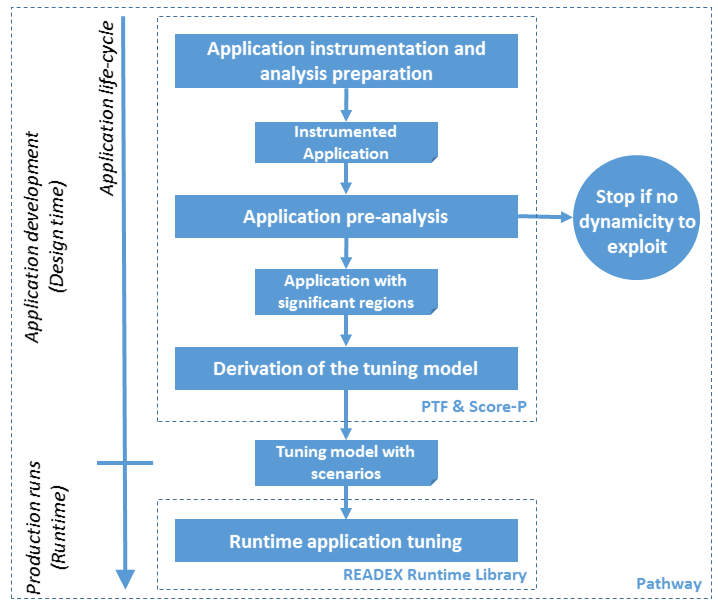
\includegraphics[width=.70\columnwidth]{figures/READEX_workflow.png}
%\caption{Overview of READEX methodology}
%\label{fig:readex_methodology}
%\end{figure}

\subsection{Application Instrumentation and Analysis Preparation}
\label{sec:application_instrumentation}
The first step in READEX is to instrument the HPC application by inserting probe-functions around different regions that are of interest to tuning. A region can be any arbitrary part of the code, for instance a function or a loop. READEX is based on instrumentation with Score-P and requires that the \textit{phase region} be manually annotated. A phase region is single-entry and exit region where most of the application progresses. Typically, a phase region may be the body of the main progress loop of the application. In addition to the phase region, READEX supports instrumentation of \textit{user regions} inside the phase region. User regions may be instrumented manually using Score-P or automatically by the compiler.

The READEX methodology also allows exposing parameters that define dynamic behaviour of the application. These parameters, referred to as additional identifiers, will enhance the distinction of different scenarios into runtime situations during the application execution, potentially leading to better identification of optimal configurations for the different tuning parameters. An example of additional identifiers is different input data sets. Exposing this information allows READEX to detect different compute characteristics of the application caused by different inputs.

\subsection{Application Pre-analysis}
\label{sec:dynamism_detection}
After instrumenting an application and preparing it for analysis, the second step in the READEX approach is to perform a pre-analysis. The objective of this step is to automatically identify and characterize dynamism in the application behaviour. This is critical because the READEX approach is based on tuning hardware, system and application parameters, depending on the dynamism exhibited by the different regions in the application. READEX is capable of identifying and characterizing two types of application dynamism:
\begin{itemize}
  \item \textit{Inter-phase dynamism}: This occurs when each phase (execution instance) of a phase region in the application exhibits different characteristics. This results in different values for the measured objective values (execution time) and thus may require different configurations to be applied for the tuning parameters.
  \item \textit{Intra-phase dynamism}: This occurs when each runtime situation (execution instance) of the significant regions in a phase region exhibits different characteristics and results in different values fo the measured objective values (execution time, compute intensity) and thus may need different configurations to be applied for the tuning parameters.
\end{itemize}
The pre-analysis also identifies the regions in the application that contribute significantly to the execution of an application and are referred to as \textit{significant regions}. If no dynamism is identified in the pre-analysis, the rest of the READEX steps are aborted due to the homogeneous behaviour of the application, which will not yield any energy or performance savings from auto-tuning.

Listing \ref{lst:minimd_dynamism_summary} presents an example of the summary of significant regions and the dynamism identified by READEX in the miniMD application.

\lstset{language=[90]Fortran,
	basicstyle=\ttfamily\scriptsize,
	frame=tb,
	aboveskip=2mm,
	belowskip=2mm,
	showstringspaces=false,
	columns=flexible,
	breaklines=true,
	breakatwhitespace=true,
	keywordstyle=\color{black},
	commentstyle=\color{black},
	escapeinside={(@*}{*@)},
}
\begin{lstlisting}[caption={Summary of Application Pre-analysis},label=lst:minimd_dynamism_summary]
...
Significant regions are:

void Comm::borders(Atom&)
void ForceLJ::compute_halfneigh(Atom&, Neighbor&, int) [with int EVFLAG = 0; int GHOST_NEWTON = 1]
void ForceLJ::compute_halfneigh(Atom&, Neighbor&, int) [with int EVFLAG = 1; int GHOST_NEWTON = 1]
void Neighbor::build(Atom&)

Significant region information
==============================
Region name                  Min(t)          Max(t)       Time Dev.(%Reg) Ops/L3miss    Weight(%Phase)

void Comm::borders(Atom&)    0.001             0.001            2.6           109              0
void ForceLJ::compute_hal    0.013             0.014            2.9            97             68
void ForceLJ::compute_hal    0.016             0.016            0.0            91              1
void Neighbor::build(Atom    0.047             0.048            0.7           332             23


Phase information
=================
Min                  Max                  Mean                 Dev.(% Phase)        Dyn.(% Phase)

0.0138626            0.0664566            0.020337             72.731               258.612

...

SUMMARY:
========

Inter-phase dynamism due to variation of execution time of phases

No intra-phase dynamism due to time variation

Intra-phase dynamism due to variation in compute intensity of following significant regions

void ForceLJ::compute_halfneigh(Atom&, Neighbor&, int) [with int EVFLAG = 0; int GHOST_NEWTON = 1]
void Neighbor::build(Atom&)
\end{lstlisting}

\subsection{Derivation of Tuning Model}
\label{sec:tuning_model_generation}

Following the identification of exploitable dynamism in the pre-analysis step, the third step explores the space of possible tuning configurations, and identifies the optimal configurations of the tuning parameters for the phases and rts's during the application execution. This analysis is performed by PTF (Periscope Tuning Framework) in conjunction with Score-P and the RRL (READEX Runtime Library). PTF performs DTA experiments through a number of possible search strategies, such as exhaustive, individual, and heuristic search based on generic algorithm to identify the optimal configurations for the rts's of the significant regions identified in the pre-analysis step that exhibit dynamism. To achieve this, Score-P provides the instrumentation and profiling platform, while the RRL provides the platform for libraries to tune hardware and system parameters. Additionally, READEX also has dedicated libraries that tune application-specific parameters.

It is important to note that the additional identifiers, which can be specified during the instrumentation step provide additional domain knowledge to distinguish and identify different optimal configurations for runtime scenarios~\cite{PACO17}.

After all experiments are completed and optimal configurations are identified, the rts's are grouped into a limited number of scenarios, e.g., up to 20. Each scenario is associated with a common system configuration, and it is hence composed of rts's with identical or similar best configurations. The limitation in the number of scenarios inhibits a too frequent configuration switching at runtime that may result in higher overheads from auto-tuning. The set of scenarios, information about the rts's associated with the scenarios, and the optimal configurations for each scenario are stored by PTF in the form of a serialized text file called the Application Tuning Model (ATM), which is loaded and exploited during production runs at runtime.

\subsection{Runtime Application Tuning}
\label{sec:runtime_tuning}

Following the completion of DTA, production runs of the application can now be tuned at runtime using the optimal configurations summarized in the ATM using the RRL. The RRL monitors the application execution using the Score-P instrumentation, identifies the scenario that is encountered at runtime, and applies the corresponding optimal configurations for each scenario using the knowledge in the ATM to optimize the application's energy consumption. The RRL uses libraries that are loaded as plugins for setting different configurations of the tuning parameters.

\subsection{Pathway for READEX Workflow}
\label{sec:pathway_for_readex_workflow}

Since the READEX methodology has quite a number of steps, it uses Pathway to automate the entire workflow. Pathway \cite{Pathway:Petkov13} is a tool for designing and executing performance engineering workflows for HPC applications. Pathway provides an out-of-the box workflow template that can be configured to apply READEX on an application in a HPC system of choice. This way, Pathway can keep track of each step that must be completed in order to obtain the tuning results. Figure~\ref{fig:pathway_browser} presents an example of a custom browser in Pathway that summarizes the results from each step of applying READEX on the miniMD application. The left pane shows the tuned applications. The top pane shows a list of experiments performed with the READEX workflow. Below are the results from the pre-analysis step, describing the dynamism detected in the application. The bottom pane displays the ATM containing the tuning results.

%\begin{figure}[!t]
%\centering
%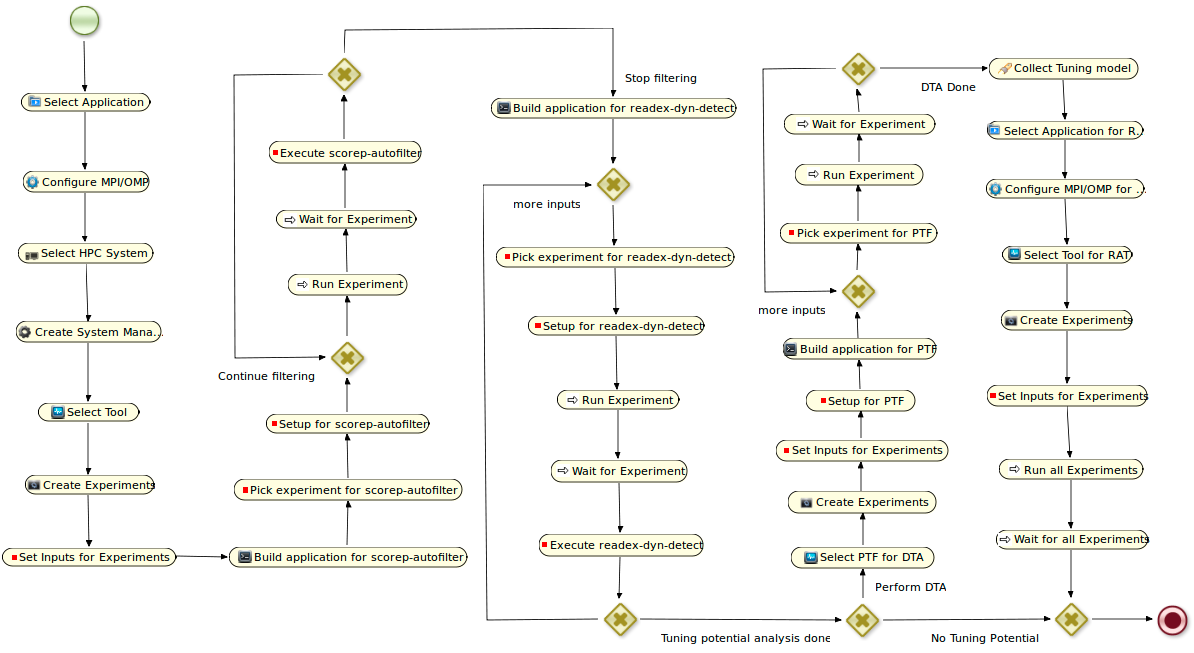
\includegraphics[width=.95\columnwidth]{figures/PathwayWorkflow.png}
%\caption{READEX Workflow in Pathway}
%\label{fig:pathway_workflow}
%\end{figure}

\begin{figure}[!t]
\centering
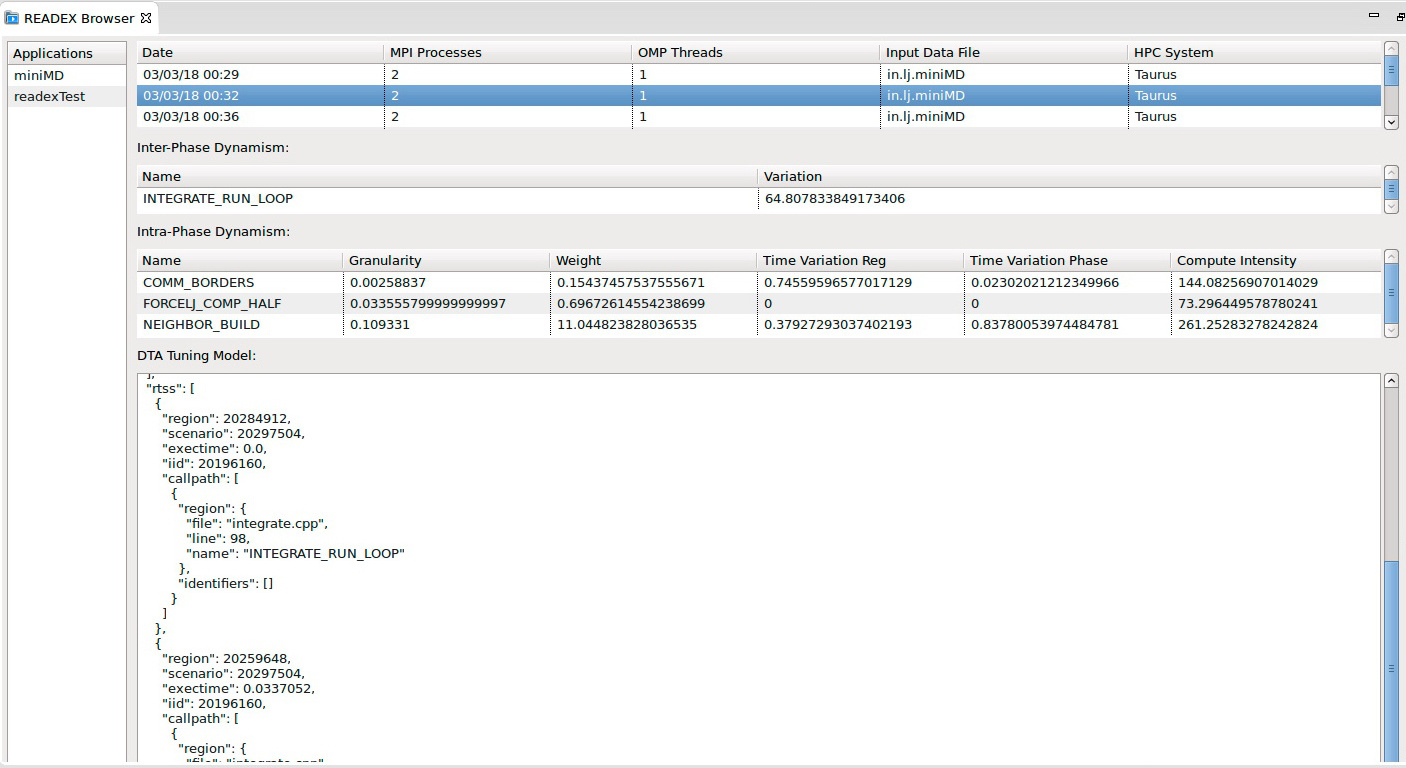
\includegraphics[width=.95\columnwidth]{figures/PathwayBrowser.jpeg}
\caption{READEX Results Browser in Pathway}
\label{fig:pathway_browser}
\end{figure}

\section{Design-Time Analysis} \label{sec:dta}
The output of readex-dyn-detect~\cite{kumaraswamy2018design} is stored in a configuration file in the \textit{xml} format. The configuration file consists of tags through which the user can provide specifications for:
\begin{itemize}
	\item Tuning parameters: Specified via the ranges (minimum, maximum, step size, and default) for two hardware parameters (CPU frequency and uncore frequency) and a system software parameter (number of OpenMP threads).
	\item Objectives: These can be the Energy, Execution Time, CPU Energy, Energy Delay Product, Energy Delay Product Squared, CPUEnergy, Total Cost of Ownership (TCO), as well as their normalized versions. The normalized versions compute the energy consumption per instruction, and can be used for applications with varying amounts of computation in a phase but no change in the phase characteristics. The total cost of ownership is the summed up cost of the energy in addition to the execution time dependent fraction for hardware and software investment as well as maintenance costs and personnel. 
	\item Energy metrics: These include the energy plugin name and associated metric names. 
	\item Search algorithm: This can be the exhaustive, random or individual search strategy. The additional parameters for each of the alogrithms can also be specified via this configuration file. Exhaustive search leads to the biggest number of configurations that are tested in subsequent program phases. The individual strategy reduces the number significantly since it is not the cross product of all tuning parameters. For this search sterategy the tuning parameters are optimized independently. With the random strategy, the number of experiments can be specified.
\end{itemize} 

DTA is performed by the Periscope Tuning Framework (PTF), which is a distributed framework consisting of the frontend, the tuning plugins, the experiment execution engine and a hierarchy of analysis agents. During DTA, PTF reads the configuration file, and calls a tuning plugin, which \todo{reference} searches the multi-dimensional space of system configurations, each of which is a tuning parameter. The tuning plugin performs one or more tuning steps, in which a user-specified search algorithm determines the set of system configurations that are evaluated. Each tuning step executes experiments to measure the effect of the system configuration on the objective. At the end of each tuning step, the plugin checks if the application should be restarted. After all the tuning steps are completed, the plugin generates tuning advice for the application.

Two new plugins, \texttt{readex\_intraphase} and the \texttt{readex\_interphase} were developed for PTF to exploit the dynamism detected by \texttt{readex-dyn-detect}. If \texttt{readex-dyn-detect} reports inter-phase dynamism for the application, the user is advised to select the \texttt{readex\_interphase} tuning plugin. Both plugins perform Dynamic Voltage and Frequency Scaling (DVFS). However, they use different approaches for DTA, and hence, it is recommended to apply the \texttt{readex\_intraphase} tuning plugin if there is no inter-phase dynamism. Sections~\ref{sec:intra-phase} and~\ref{sec:inter-phase} describe in details the steps performed by the \texttt{readex\_intraphase} and \texttt{readex\_interphase} plugins to exploit the application dynamism.


\subsection{Intra-Phase Plugin} \label{sec:intra-phase}

PTF performs intra-phase dynamism tuning by executing \textbf{readex\_intraphase} plugin when there is no changes of the dynamic characteristics across the sequence of phases.  

The \textbf{readex\_intraphase} plugin is executed in four tuning steps: default execution, ATP tuning, system parameter tuning and the verification step. The default exection is the computation of the objective value for the default paramter settings. Next, the ATP tuning investigates optimal settings for the given ATPs. The application is tuned with the optimal ATP settings along with the system level parameters during the system parameter tuning step. The verification step analyzes the results of the previous step and determines the best system configuration for the phase region as well as the specific best settings for the rts's.

\subsubsection{Default Execution} \label{intra-default-execution} 

During this step, PTF executes the plugin with the default configuration of the tuning parameter to collect the program's static information after starting the application. The default settings are provided by the batch system for the system parameter and the ATP specification in the code for ATPs. PTF uses a specific analysis strategy to gather program regions and runtime situations only for the first phase of the application. The measurement results are required to evaluate the objective value, for example, time and energy and stored to compare with the results of the verification step.

\subsubsection{ATP Tuning} \label{atp-tuning} 
The next step is to tune ATPs as they are specifically independent of the system-level tuning parameter. The application expert can provide such kind of application specific parameters for example algorithmic choices. The detail about ATP is described in section ~\ref{sec:atp}. 

The plugin provides two new search strategies, \textbf{exhaustive\_atp} and \textbf{individual\_atp} to compute the optimal ATP configuration. These two search strategies can also be configured via the READEX configuration file.

The \textbf{exhaustive\_atp} search space is built from the crossproduct of all valid combinations of ATPs. The plugin contacts to the ATP server to receive the valid combinations of the points for each of the given ATP domains. The configuration set   is then built from the cross products of the computed valid points. 

On the other hand, the \textbf{individual\_atp} stratgey is computed from the domains individually instead of the crossproduct of the valid points of the domains. It first evaluates all valid points for the first domain. The best point from this domain remains fixed and the next domain is investigated until all the domains were explored. The search strategy then used \textbf{exhaustive\_atp} to explore the valid points of a domain. 

\subsubsection{System Parameter Tuning} \label{sys-tuning} 
The system-level parameter tuning investigates the optimal configuration for system-level tuning paramter keeping the optimal configuration of the ATPs fixed found during the previous step. The search strategy is read from the configuration file. If no strategy is specified, the default individual search algorithm is selected on this step. The experiments are created for all possible ranges of the system-level tuning parameters. The plugin evaluates the objective for the phase region followed by for each rts to compute the best system configuration respectively. The READEX tuning model is generated from this knowledge. 

\subsubsection{Verification} \label{intra-verification} 
The verification step is performed by executing additional three experiments in order to check for phase variations with the results produced in the previous step. For this purpose, PTF configures RRL with the best system configuration for phase region and with the rts-specific best configuration. RRL switches system configurations dynamically for the rts's. 

Finally, the plugin determines the static and dynamic savings for the rts's ans static savings for the whole phase to evaluate the tuning result and then a tuning model is precomputed. Additionally, the generated tuning model for differents inputs of an application can be merged into one general tuning model by an external \textbf{Tuning Model Merger} tool. The detail about this tool is explained in section~\ref{sec:input}. 
 
\subsection{Inter-Phase Plugin} \label{sec:inter-phase}
The \texttt{readex\_interphase} plugin \todo{reference} is used for tuning applications that exhibit inter-phase dynamism, where the execution characteristics change across the sequence of phases. While the \texttt{readex\_intraphase} plugin does not consider similarities in the behavior between different phases, the \texttt{readex\_interphase} tuning plugin first groups similarly behaving phases into clusters, and then determines the best configuration for each cluster. It also determines the best configurations for the rts's of each created cluster.

The \texttt{readex\_interphase} plugin performs three tuning steps: cluster analysis, default execution and verification to first cluster the phases, then execute experiments for the default setting of the tuning parameters, and finally, verify if the theoretical savings match the actual savings incurred after switching the configurations. Sections~\ref{cluster-analysis},~\ref{default-execution} and~\ref{verification} describe the tuning steps in detail.

\subsubsection{Cluster Analysis} \label{cluster-analysis} 
The plugin first reads the significant regions, ranges of the tuning parameters and the objectives from the READEX configuration file. It then uses the random strategy to create a user-specified number of experiments. In each experiment, the plugin measures the effect of executing a phase with a random system configuration from a uniform distribution \todo{reference} on the objective value. The plugin also requests for PAPI hardware metrics, such as the number of AVX instructions, L3 cache misses, and the number of conditional branch instructions, which are used to derive the features for clustering.

Features for clustering are selected carefully, as they have a high impact in selecting the cluster-best configuration. Since the dynamism in many applications results from the variation in the compute intensity and the number of conditional branch instructions, they were chosen as the features for clustering. The compute intensity is defined by $\frac{\#AVX Instructions}{\#L3 Cache Misses}$. The plugin first normalizes the features and the objective values for all the phases and the rts’s by a metric which is representative of the work done, such as the number of AVX instructions. It then transforms the numeric range of the features to [0,1] scale using min-max normalization.

The plugin then groups points that are closely packed together into clusters, and marks points that lie in low-density regions and have no nearby neighbors as noise using the DBSCAN (Density-Based Spatial Clustering of Applications with Noise) algorithm \todo{reference}. DBSCAN is a density based clustering algorithm, which requires the \textit{minPts} and the \textit{eps} parameters to cluster the phases. \textit{minPts} is the minimum number of points that must lie within a neighborhood to belong in a cluster, and is set to 4 \todo{reference}.\textit{eps} is the maximum distance between any two data points in the same neighborhood, and is automatically determined using the elbow method \todo{reference}. The elbow is a sharp change in the average 3-NN Euclidean distances plot, and represents the point that has the maximum distance to the line formed by the points with the minimum and maximum 3-NN distances.

The plugin then selects the best configuration for each cluster based on the normalized objective value. The cluster-best configuration represents one best configuration for all the phases of a particular cluster, and individual best configurations for the rts's in the cluster.

\subsubsection{Default Execution} \label{default-execution} 
The tuning plugin restarts the application and generates the same number of experiments as the previous tuning step. In each experiment, the phase is executed with the default system configuration, i.e., the execution with the default parameter settings provided by the batch system for the system tuning parameters. The plugin uses the objective values obtained for the phases and the rts’s to compute the savings at the end of the tuning plugin.

\subsubsection{Verification} \label{verification} 
The plugin restarts the application executes the same number of experiments as the previous tuning steps. In each experiment, the plugin executes the phase with the
corresponding cluster-best configuration and the rts's with their rts-specific
best configurations. Phases that were noise points in the clustering step are executed with the default configuration.

The plugin first creates a new node for each cluster, and then clones the children of the phase region of the Calling Context Graph (CCG) \todo{reference}. It stores the tuning results, including the measured objective values and the ranges of the features for the cluster in each node. 

\subsection{Computational Savings} \label{sec:com-savings}
Both plugins compute the following three values to characterize the savings at the end of the execution:
\begin{enumerate}
	\item Static savings for the rts's: The total improvement in the objective value with the static best configuration of the rts’s over the default across all the clusters.
	\item Dynamic savings for the rts’: The total improvement in the objective value for the rts’s with their specific best configuration over the static best across all the clusters.
	\item Static savings for the whole phase: The total improvement in the objective value for the best static configuration of the phase over the default across all the clusters.
\end{enumerate}

%The tuning model contains the list of clusters generated by the clustering algorithm, the set of phases belonging to each cluster, the ranges of the features that were used for clustering, the list of rts's that were tuned by the plugin, the scenarios into which they are classified, and the best configuration for each scenario.


\section{Tuning Model Generation} \label{tm-generation}
\textbf{NTNU (2 pages)}

\textcolor{blue}{\begin{enumerate}
    \item Creation of scenarios to reduce switching overhead
	\item How does the selector work 
  	\item Cost function / trade-off 
\end{enumerate}
}


\section{Tuning Model Visualization} \label{tm-visualization}
\textbf{TUM (1 page)}
\section{Runtime Application Tuning} \label{rat}

The Runtime Application Tuning (RAT) phase of READEX is carried out by the low-overhead READEX Runtime Library (RRL). The RRL is implemented as a Score-P Substrate Plugin. The plugin interface allows to utilize the instrumentation infrastructure of Score-P, without direct integration into Score-P~\cite{Schoene2017}. This approach reduces maintenance and integration efforts by keeping the RRL as a separate entity. As a substrate plugin, the RRL receives notifications for different instrumented events that occur during runtime. It uses this information to make switching decisions based on the application tuning model created at design-time.

The RRL implements three main mechanisms in order to apply the dynamic configuration switching at runtime: scenario detection, configuration switching, and calibration. The following sections detail the first two mechanisms, while Section~\ref{sec:calibration} describes the calibration mechanism, which is an extension to the standard version that only relies on the previously written ATM.

%\begin{figure}[!t]
%\centering
%%\includegraphics[trim={7cm 2cm 5.5cm 2cm},clip,width=3in]{readex-approach}
%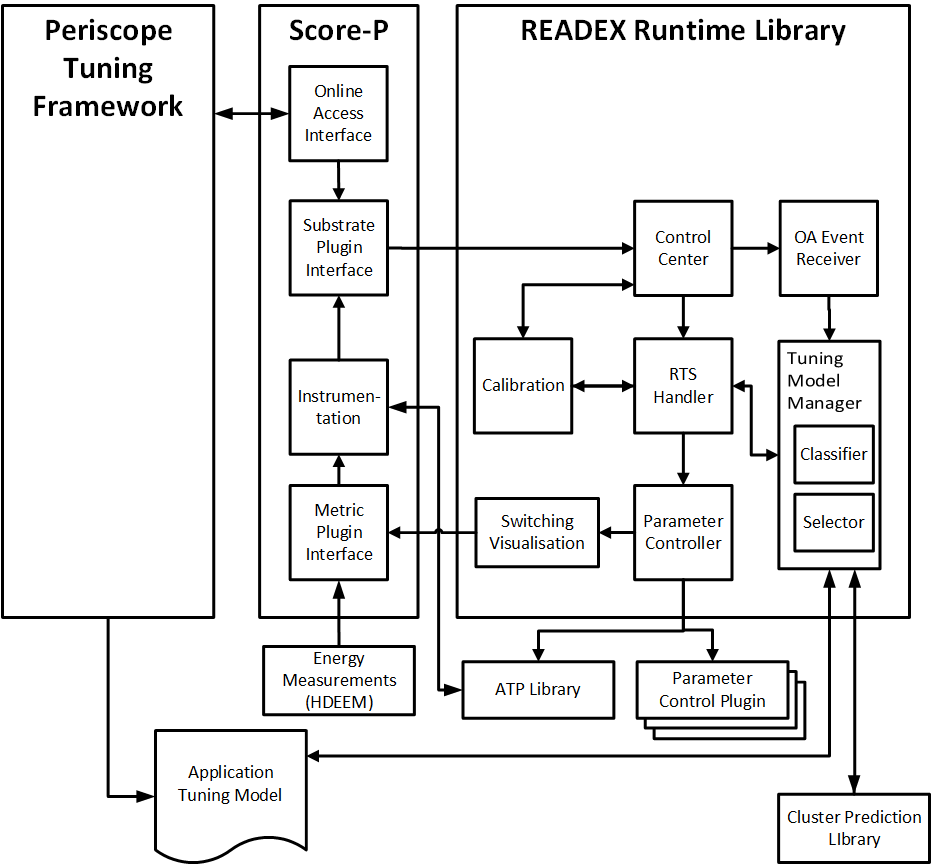
\includegraphics[width=.8\columnwidth]{figures/RRL_Architecture.png}
%\caption{Architecture of the READEX Runtime Library (RRL)}
%\label{fig:rrl}
%\end{figure}

\subsection{Scenario Detection}\label{scenario-detection}
Runtime detection of the upcoming scenario involves several steps. First, the ATM is loaded during the application start. Here, the RRL reads the set of configurations, in the form of scenarios, classifiers, and selectors. When an application region is entered during the execution, the RRL receives a notification of a region enter event from Score-P, and performs a check to detect if the encountered region is significant by searching for the region in the ATM. If the region is found, it is marked as a significant region. Otherwise, it is marked as an unknown region. 

Another check is performed to determine if the region must be tuned by computing the granularity of the region. The region will be tuned only if the granularity is above a specified threshold, which defaults to 100\,ms. Once the region is determined to be both significant and coarse-granular enough, additional identifiers that are used to identify the current rts are requested. The current rts can then be identified by both the call stack and the additional identifiers. Finally, a new configuration is applied for the current rts to perform the configuration switching.
For a coarse-granular region that is marked as unknown, the calibration mechanism is invoked.

\subsection{Configuration Switching}\label{config-switching}
The scenario detection step applies a new configuration to the current region only if the region entered is found to be significant and coarse-granular. The setting for each tuning parameter is controlled by a dedicated Parameter Control Plugin (PCP). The RRL switches a configuration by sending a request to the PCPs. 

The RRL supports two different modes for configuration switching: \textit{reset} and \textit{no-reset}. The \textit{reset} mode maintains a configuration stack. Whenever a new configuration is set, the previous configuration is pushed onto this stack. When the corresponding unset occurs (e.g., if an instrumented region is left), the element is removed from the stack and the previous configuration is re-applied. If the \textit{no-reset} mode is selected, the current configuration remains active until a new configuration is set, and the unset is ignored. This behaviour is configurable by the user. By default, the \textit{reset} mode is enabled.

\subsection{Calibration}\label{calibr}
READEX makes a distinction between seen and unseen rts's. For known or seen rts's that are already present in the ATM, RRL simply uses the optimal configuration, and performs configuration switching. For the unseen rts's, the RRL calibration mechanism, described in Section~\ref{sec:calibration} is used to find the optimal system configuration based on machine learning algorithms.

 
%Before the current region exits, the RTS Handler receives the notification  from Score-P through Control Center. The RTS Hander checks if the current region was set up for calibration. If yes, it requests the configuration for the currently exited region from the
%Calibration module. Once the RTS handler gets back the configuration from the calibration module, it passes this configuration to the TMM which stores the new configuration for the respective rts. If the region was not set up for calibration, then the Parameter Controller is informed that it might want to unset the current configuration. 

 
\section{Dynamic Switching Visualization} \label{switching-visualization}
During DTA, PTF runs experiments with different configurations to find the optimal configuration for each rts in the application, which are then stored in the tuning model. During RAT, the RRL applies the optimal configuration from the tuning model for each rts during the application run. Hence, both stages require configuration switching during the application run.

To enable the user to visualize the configuration switching for each region during DTA and during a production run, a switching visualization module is included in the RRL. 
The visualization module is implemented as a Score-P metric plugin, which uses the Metric Plugin Interface provided in Score-P~\cite{Schoene2017}. The user can select any of the hardware, software and application tuning parameters to visualize the switching pattern. The tuning parameter selection is configurable, and the user can specify if all the tuning parameters or a subset has to be recorded. Each of the tuning parameters is then added as a metric and recorded in a trace in the \textit{OTF2} format~\cite{otf2} by Score-P. The trace can be visualized in Vampir~\cite{BHJR:10:VampirOverview}. 

\begin{figure}[!t]
	\centering
	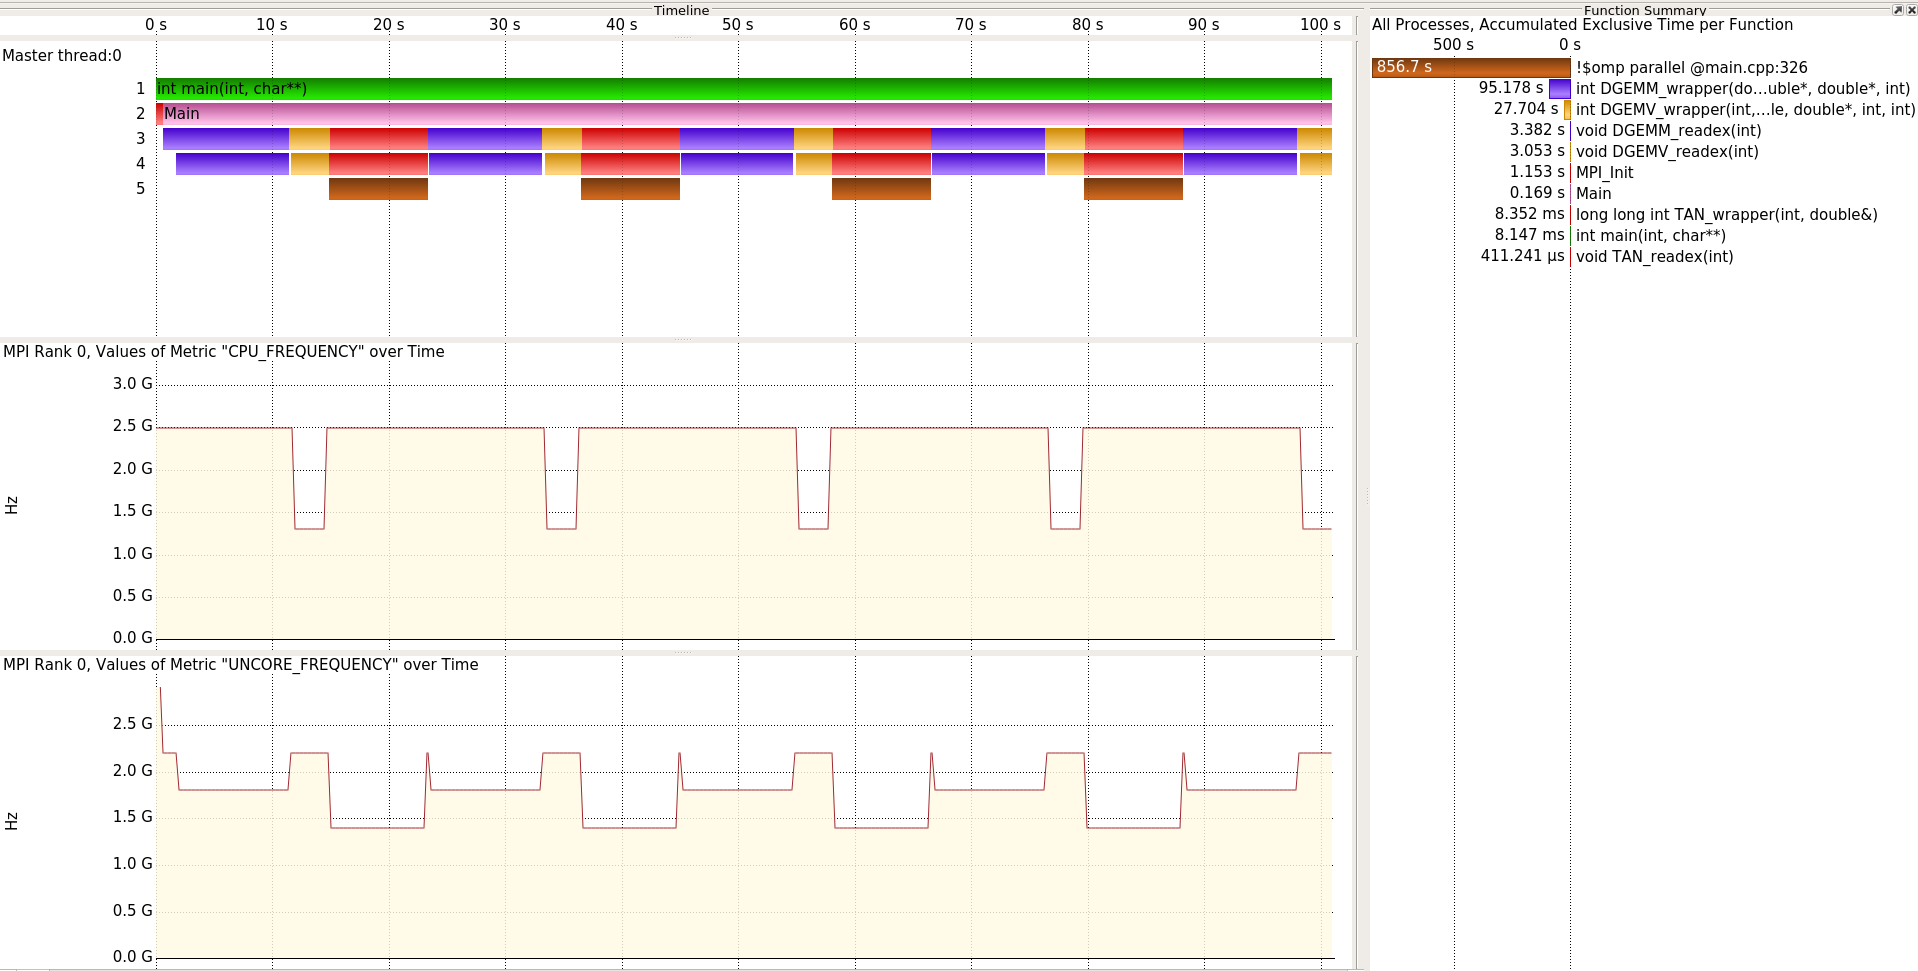
\includegraphics[width=.97\columnwidth]{figures/visualization_trace.png}
	\caption{{CPU\_FREQUENCY} and {UNCORE\_FREQUENCY} switchings during Blasbench runtime tuning}
	\label{fig:switch_visualization}
\end{figure}
 
Figure~\ref{fig:switch_visualization} illustrates the switching of the CPU frequency and uncore frequency tuning parameters performed by RRL while tuning the Blasbench benchmark. The top timeline shows the call stack of the application regions. Below that, we see the CPU frequency changing from 2.5 GHz to 1.3 GHz. Finally, the bottom pane shows the switching of the uncore frequency according to the optimal settings of the different regions.
%\newpage

 
\section{Extensions} \label{sec:extensions}
\textcolor{blue}{1. Extensions to the standard version}






\subsection{Application Tuning Parameters} \label{sec:atp}
\textbf{Intel (1 page)}
\textcolor{blue}{\begin{enumerate}
	\item Motivation
	\item How does this work? (A high level workflow, maybe?)
	\item Explain that ATPs are combined to domains and those in a domain can have constraints. 
	\begin{itemize}
		\item Manual insertion into code (ATP library). Can use runtime info to set e.g. the value space of an ATP.
		\item Pre DTA: Generation of ATP file
		\item During DTA: ATP server providing valid settings for ATPs based on the value space and the constraints.
		\item During RAT: Read by ATP library from the RRL
	\end{itemize}
\end{enumerate}}
\subsection{Application Configuration Parameters} \label{sec:acp}

Application level tuning parameters are frequently given in the input files configuring the program run. To simply tuning those Application Configuration Parameters (ACP) READEX provides an additional tuning plugin. 

The \texttt{readex\_configuration} tuning plugin enables tuning of ACPs with respect to one of the objectives supported by READEX. The plugin first reads a plugin specific configuration file. This specifies the objective, the search algorithms, and the tuning parameters. ACPs are identified by their name in the input file. For each such input file a template file with the name is given. During the search for the optimal configuration for the ACPs, the plugin copies the template file to the input file and replaces all ACP names with the value given in the selected configuration. It then restarts the application and measures the resulting objective value for the phase region. Only a single phase is required, but also a burst of phases can be used in the experiment. The READEX User's Guide in the appendix provides details of this procedure. 

The final outcome of this tuning plugin is an optimal configuration for the ACPs which is output into a file. Furthermore, final input files are created from the template files by replacing ACPs by their value in the best configuration.  

\subsection{Input Identifiers} \label{sec:input}
\textbf{TUM and NTNU (1 page)}
\textcolor{blue}{
\begin{enumerate}
	\item Motivation
	\item Explain how input identifiers are given in separate file.
	\item Talk about handling of processes/threads
	\item Tuning model merging
\end{enumerate}}
DTA is executed to observe the characteristic variations for different input sets. This helps the user to improve the tuning model by identifiying more rts's due to variations in application executions. The application executions are identified via input identifiers in the form of key-value pairs in a separate file. For example, in the MG benchmark, different grid sizes may change the compute intensity characteristics while switching to different grid levels. As the optimal configuration changes due to this switching, grid size is considered as a part of input identifier. In addition to grid size, number of processes also changes the compute intensity characterisitic. As the number of processes increase, data distributes better over the caches which results switching between memory bound and compute bound. So the numbers of processes are also considered as input identifiers

Each input identifier is attached to a specific ATM while generating tuning model at the end of the \texttt{readex\_intraphase} plugin. In order for all of the tuning information from the different ATMs to be usable by the RRL, these tuning models must be merged into a single tuning model. This is the task of the tuning model merger.

The tuning model merger is a standalone program that takes all the ATMs as input on its command line and outputs a new ATM incorporating all the rts's from the input ATMs. The program does this by first deserializing all ATMs. It extracts all tuning information from the ATMs, such as rts's and their system configurations as well as the corresponding input identifiers. The scenarios from the individual ATMs are discarded. Next the tuning model merger filters all rts's in order to avoid duplicated rts's in the final tuning model. The next step is to produce a new set of scenarios by clustering all rts's as described in Section \ref{tm-generation}. Finally, the tuning model merger serializes the merged tuning model information and outputs the new ATM in the JSON format.

\subsection{Runtime Calibration} \label{sec:calibration}
During RAT, we differentiate between known and unknown rts's. 
Known rts's are those which have been encountered during DTA. So the optimal configuration for the rts's is known. 
However, unknown rts's describe those which have not been encountered during DTA. 
There are several reasons why unseen rts's might occur. 
First, an unseen rts may consists of already known regions, but with unknown user parameters that were not present during DTA or parameters that might have changed between DTA and runtime. Typically, these changes are related to different application inputs. 
Second, an unseen rts may consist of completely new regions, which were not seen during DTA. 
The goal of the calibration is to handle these unknown rts's during RAT.

Since, the calibration is done during the production run, there are a few restrictions which had to be taken in account for the design of calibration mechanism. 
First, there can be no user input and 
second, a good configuration has to be found in short time. 
A DTA like approach for searching optimal configuration is not feasible as it would degrade the performance of the application.
To avoid this a Machine Learning based method is used to
determine a good configuration for an unseen rts. 
Using this method we could split the calibration in a training part and a detecting part. 
The training is done once per HPC system and described below. During RAT the trained model is used to detect a good configuration.
Once a configuration is found, it is stored in the TMM.

\subsubsection{Data Basis:}
Each Machine Learning algorithm needs a data basis, also called \textit{feature vector}, to learn from. 
For supervised learning, an \textit{optimization criterion} and a \textit{target vector} are needed as well. 
In our case, the \textit{optimization criterion} is to reduce the energy consumption of certain program functions. 
To do so, we change the frequency of the processor core and uncore, which represents the \textit{target vector}. 
The training examples are generated by different energy optimal frequencies for monitored program functions. 
As feature vector, we use the hardware performance measurement counters (PMCs) as the data basis to learn from and predict a
good configuration.

PMCs are CPU registers that can be used to count different hardware events, like executed instructions, cache accesses, and branch predictions.
Modern processor architectures are equipped with counters that measure events related to the processing units and core-related caches, and counters that observe the behavior of shared components within the uncore \cite{molka:2017:a}.
A detailed description for core and uncore counters on the Intel
Haswell-EP platform can be found in \cite{Intel2018} and \cite{xeon_e5v3_Uncore}, respectively.

The purpose of the learning algorithm is to use these counters to predict the most energy efficient configuration of the processor frequency for a specific region. However, as there is only a limited number of PMCs available to measure the different events, it is not possible to collect all events at the same time. Hence, we need to find the appropriate core and uncore events.

\subsubsection{Selecting Relevant Performance Events:}

Suitable hardware events are those that contribute to a decision about the optimal frequencies.
However, to gain the most accurate information, we need to filter out redundant information. 
We use the \textit{Correlation-based feature selection} approach proposed by Yoo \cite{Yoo2012} to choose events without reduntant information. 
To generate the input vectors for the learning algorithm, we remeasure
the chosen relevant events to generate new feature vectors.

\subsubsection{The Learning algorithm:}
For the implementation of the learning algorithm we chose Neural Networks (NN). 
Neural networks try to mimic the human brain, where computational units often referred to as \textit{neurons} combine input values to produce an output value \cite{Haykin2009}.
The aim is to collect feature vectors for a given configuration of the processor frequency that results in the lowest energy consumption. Moreover, in the training step, this data is normalized by the runtime of the region and used as input to the NN. The optimal processor
frequency for each region is termed as output.

\subsubsection{Training and Runtime:}
For tuning of the ML algorithm, the PTF is replaced by the tuning framework in Figure~\ref{fig:rrl} and PMCs are given as input. 
For training, SPEC OpenMP benchmark has been used. The benchmarks are run on our target platform \ref{sec:results} and different performance counters are collected. 
At the end of each benchmark run, the collected counter
data is saved and evaluated by the training framework. 
If the collected counter data are sufficient, the framework will proceed. Otherwise, the benchmark is executed again. 
Once the training satisfies the quality requirements set, the framework determines which events are the most interesting ones.

Now, at runtime during a production run, when the RTS-Handler
detects the presence of an unseen rts, instead of using a system configuration found during DTA, the calibration module specifies a configuration and starts collecting values from the pre-selected set of counters.
At a pre-determined point in the program, for example, after 100 iterations, the collected counter values are fed to the learning algorithm, which then determines the best configuration to apply for future occurrences of the same rts.
\section{Results} \label{sec:results}
%%%%%%%%%%%%%%%%%%%%%%%%%%%%%%%%%%%%%%%%%%%%%%%%%%%%%%%%%%%%%%%%%%%%%%%%%%%%%%%%%%%%%%%%%%
%\textbf{IT4I (3 pages)}
%\textcolor{blue}{\begin{enumerate}
%	\item Description of the machine/modules
%	\item Rational behind selecting application classes, i.e., benchmarks, proxy apps, applications
%	\item Brief description of the dynamism in the selected applications
%	\item Add the results that were presented at the review meeting. Focus on the table presenting the overall results and not specifically to a single application. 
%	\item Do not compare to the project goals but present the achievements. e.g. min, max, avg compared to manual tuning. 
%	\begin{itemize}
%		\item A table summarizing the savings - improvements
%		\item Should add inter-phase results to this - TUM
%		\item Describe the overall effect of using the READEX methodology
%	\end{itemize}
%	\item Results for ATPs
%\end{enumerate}}
%%%%%%%%%%%%%%%%%%%%%%%%%%%%%%%%%%%%%%%%%%%%%%%%%%%%%%%%%%%%%%%%%%%%%%%%%%%%%%%%%%%%%%%%%%
\subsection{Description of the machine/modules}
To demonstrate that READEX is capable of supporting different architectures and software stacks, we test it on the Intel Haswell and Intel Broadwell processors both at TU Dresden's Top500 cluster Taurus. Taurus' Haswell (two Xeon E5-2680 v3 on a single node, 12 cores each) partition has been selected especially due to reliable power measurement infrastructure called HDEEM~\cite{hdeem} that was used for energy measurement in this project. For energy measurements on Broadwell (two Xeon E5-2680 v4, 14 cores each) partition we used Intel RAPL counters with 75\,W baseline~\footnote{The Broadwell's baseline has been established based on low frequency measurements from IPMI.} to measure not only the CPUs but the energy consumption of the whole node as well as in case of HDEEM.

%Another site where we did the tests is Haswell (two Xeon E5-2680 v3 on single node, 12 cores each) based cluster Salomon operated by IT4Innovations national supercomputing center, in this case the Intel RAPL counters had been used for energy measurement. Taurus as well as Salomon system are listed in the Top500 list most power-full supercomputers.

%%%%%%%%%%%%%%%%%%%%%%%%%%%%%%%%%%%%%%%%%%%%%%%%%%%%%%%%%%%%%%%%%%%%%%%%%%%%%%%%

\subsection{Rational behind selecting application classes, i.e., benchmarks, proxy apps, applications}
Following text presents the energy savings that have been achieved when using READEX tools. The list of the application is based on READEX test apps, it consists of three basic benchmarks, Kripke, Lulesh and Blasbench, that had been selected to show and test the tools functionality. Rest of the suite are fully-fledged applications. Since BEM4I and ESPRESO results are presented into further details, it should be briefly introduced. 

BEM4I~\cite{ch6_MerZap2013} is a solver for partial differential equations based on the boundary element method and is under development at IT4Innovations. Contrary to finite element solvers, BEM4I produces dense matrices and due to the nature of boundary integral equations the assembly of system matrices is more or less compute bound. This is in contrast to the iterative solver used for the solution of the resulting system of linear equations which is usually memory bound due to matrix vector multiplications. BEM4I is thus a suitable library to be involved in the test apps repository.

The ESPRESO library~\cite{ESPRESOijhpca} is a combination of Finite Element (FEM) and Boundary Element (BEM) tools and TFETI/HTFETI solvers. It supports FEM and BEM (uses BEM4I library) discretization for Advection-diffusion equation, Sto\-kes flow and Structural mechanics. The ESPRESO solver is a parallel linear solver, which includes a highly efficient MPI communication layer designed for massively parallel machines with thousands of compute nodes. The parallelization inside a node is done using OpenMP.


\subsection{Add the results that were presented at the review meeting. Focus on the table presenting the overall results and not specifically to a single application. Do not compare to the project goals but present the achievements. e.g. min, max, avg compared to manual tuning.}

Table~\ref{tab:overall2} shows how the runtime and energy consumption changed, when the READEX toolsuite was applied to tune the selected applications. Achieved energy savings varies between 4.3\,\% and 34\,\%. 

\begin{table}[h]
    \centering
%	\resizebox{\textwidth}{!}
%	{%

    \begin{tabular}{|c|c|cH|}
    \hline
            &       Broadwell &         Haswell &         IT4I HSW \\
            &     energy/time &     energy/time &      energy/time \\ \hline
AMG2013	    &   7.5\%/-10.5\% &   7.0\%/-14.0\% &   3.4\%/-23.2\%  \\ \hline
Blasbench   &  12.0\%/-19.0\% &   9.9\%/ -9.2\% &  10.9\%/-19.8\%  \\ \hline
Kripke	    &   4.3\%/-10.3\% &  10.5\%/-28.9\% &  10.3\%/-22.2\%  \\ \hline
Lulesh	    &  10.0\%/ -9.2\% &  18.2\%/-25.7\% &   7.3\%/-20.6\%  \\ \hline
BEM4I	    &  23.0\%/ -1.1\% &  34.0\%/ 10.9\% &  24.3\%/  8.2\%  \\ \hline
INDEED	    &  14.0\%/-18.0\% &  19.1\%/-17.3\% &             -    \\ \hline
NPB3.3-BT-MZ&   8.9\%/-11.3\% &  10.8\%/-12.0\% &   3.1\%/ -2.8\%  \\ \hline
ESPRESO	    &           -     &   7.1\%/-12.3\% &   8.1\%/ -7.0\%  \\ \hline
OpenFOAM    &   7.5\%/ -7.6\% &   9.8\%/ -9.8\% &  18.4\%/ -7.5\%  \\ \hline
    \end{tabular}

%	}
    \caption{Overall time and energy saving that has been achieved when READEX tools has been applied on the applications, comparing the results on Broadwell and Haswell platforms.}
    \label{tab:overall2}
\end{table}


The BEM4I library shows the best energy savings from the evaluated applications, and in case of the evaluation at Haswell nodes the tuned runs were also shorter than the runs without tuning.


\subsection{Brief description of the dynamism in the selected applications}
Partial Differential Equations (PDEs) are often used to describe phenomena such as sheet metal forming, fluid flow, and climate modeling. One of the numerical approaches to solving PDEs is the boundary element method (BEM) implemented, e.g., in the BEM4I library. In contrast to volume based methods, such as the finite element/differences/volume methods, BEM gives dense matrices whose assembly results in a compute bound code. This fact is even more pronounced when the assembly kernels are parallelized and vectorized as in the case of BEM4I~\cite{ch6_ZapMerMal2016,ch6_MerZapJar2016}. On the other hand, the iterative GMRES solver based on the matrix-vector product as implemented in the Intel Math Kernel Library (MKL) is much less compute intensive and results in memory bound computation. Furthermore, printing the results for visualization leads to an I/O bound region. 

For the memory bound solver (GMRES) the manual tuning results in a low core frequency, high uncore frequency and use of eight threads to overcome non-uniform memory access (NUMA) effects of the dual socket computational node. While static savings reach 15.7~\%, the dynamic switching among individual configurations increases the savings to 34.0~\% at the Haswell nodes. Decrease in runtime in this case is caused by NUMA effects of the MKL solver -- the tuned version runs on eight threads and due to the compact affinity all threads run on a single socket.
The energy and time consumption of each region in the application in optimum static and optimum dynamic (optimum configuration for the region itself) configuration is presented in Table~\ref{tab:BEM4Idynamicity2}, from which we can see that the optimum static configuration has very bad impact on assemble\_k and assemble\_v regions, also behavior or the region print\_vtu is suboptimal.

%\begin{table}[h]
%    \centering
%    \begin{tabular}{|c|c|c|c|c|c|}
%    \hline
%Compute node energy &	assemble\_k & assemble\_v & gmres\_solve & print\_vtu & main  \\ \hline
%default energy  	&	1467\,J &	1484\,J &	2733\,J &	1142\,J &	6872\,J \\ \hline
%static tuning energy&	1962\,J &	2015\,J &	1366\,J &	 420\,J &	5792\,J \\ \hline
%dynamic tuning energy&	1476\,J &	1462\,J &	1259\,J &	 293\,J &	4531\,J \\ \hline
% \hline
%\textbf{static savings}  	&	-33.8\%	& -35.8\% & 50.0\% & 63.2\% & 15.7\% \\ \hline
%\textbf{dynamic savings} 	&	-0.6\%	&   1.5\% & 53.9\% & 74.3\% & 34.0\% \\ \hline
%    \end{tabular}
%    \caption{Comparison of the BEM4I regions energy consumption in the application default, optimal static and dynamic configurations.}
%    \label{tab:BEM4Idynamicity}
%\end{table}

\begin{table}[h]
    \centering
	\resizebox{\textwidth}{!}
	{%
		\begin{tabular}{|c|c|c|c|c|c|}
		\hline
			 &	assemble\_k & assemble\_v & gmres\_solve & print\_vtu & main \\ 
			 & [J]/[s]     & [J]/[s]    & [J]/[s]     & [J]/[s]   & [J]/[s] \\ \hline
		default setings	&	1467/5.4 &	1484/ 5.9 &	2733/10.2 &	1142/5.6 &	6872/27.3 \\ \hline
		static tuning	&	1962/9.8 &	2015/10.6 &	1366/ 6.1 &	 420/2.4 &	5792/29.0 \\ \hline
		dynamic tuning	&	1476/7.0 &	1462/ 7.2 &	1259/ 7.9 &	 293/2.1 &	4531/24.3 \\ \hline
		 \hline
		static savings [\%]  & -33.8/-82.3	& -35.8/-79.1 & 50.0/40.5 & 63.2/56.8 & 15.7/-6.2 \\ \hline
		dynamic savings [\%]	&  -0.6/-30.6	&   1.5/-20.9 & 53.9/23.2 & 74.3/62.9 & 34.0/10.9 \\ \hline
		\end{tabular}
	}
    \caption{Comparison of the BEM4I regions time and energy consumption in the application default, optimal static and dynamic configurations.}
    \label{tab:BEM4Idynamicity2}
\end{table}



\subsection{Application Parameters tuning}
As mentioned in the previous sections READEX comes with two approaches to tune application parameters: (1) using the ATP library and (2) using Application Configuration Parameters (ACP). The integration of the ATP library requires developer knowledge of the application and therefore, we implemented this support into the ESPRESO library, that is developed by one of the partners (IT4Innovations) in the READEX project.

There is a long list of application parameters that were evaluated: runtime tuning of FETI METHOD (2 options), PRECONDITIONERS (5 opts.), ITERATIVE SOLVERS (2 opts.), HFETI type (2 opts), SCALING (2 opts), BO\_TYPE (2 opts), NON-UNIFORM PARTS (6 opts), REDUNDANT LAGRANGE (2 opts.) and adaptive precision (2 opts.). For runtime tuning of domain decomposition (10 opts.) a developer had to implement the support for this parameter, since ESPRESO performs domain decomposition only during startup. For the READEX project, we developed enhanced ESPRESO to redo the decomposition after each time-step of a transient simulation. Total number of possible combinations is 3840.

There is no default configuration in ESPRESO. Based on the problem that is being solved, a user has to setup the FETI solver in ESPRESO based on his knowledge of the problem he wants to solve, so we cannot present savings against default configuration, just compare the consumption in the best and the worst case. The worst case scenario took 1320 seconds and consumed about 230 kJ, on the other hand the best case scenario consumed 32.5 kJ in 189 seconds. Comparing these two cases gives us 86\% energy savings. If user would specify some reasonable settings, the energy consumption might be about 50-66\% higher than in the best possible settings.

Besides the ESPRESO library we have analyzed another three libraries using ATP or ACP, the results in energy savings are presented in Table~\ref{tab:ATPACP}.

\begin{table}[h]
    \centering

    \begin{tabular}{|c|c|c|c|}
    \hline
Application & \# parameters tested /& Energy savings     & Energy savings \\
            & total \# of options      & vs. worst settings & vs. default* settings\\
\hline
ESPRESO     & 9/3840 & 86\% & 50--66\% \\ \hline
ELMER       & 1/40   & 97\% & 50--75\% \\ \hline
OpenFOAM    & 2/12   & 24\% &      8\% \\ \hline
INDEED      & 3/12   & 35\% &     25\% \\ \hline

    \end{tabular}
    \caption{Table of application that has been evaluated with READEX ATP/ACP, shows the difference in energy consumption in optimal settings compare to worst settings and default one. *If default settings is not available, the values refer to any reasonable settings.}
    \label{tab:ATPACP}
\end{table}




\section{Conclusions} \label{sec:conclusions}

The READEX project developed a tool suite for dynamic tuning of the energy efficiency of HPC applications. It pre-computes during design-time a tuning model that is then passed to the runtime for switching system configurations when certain regions start. This dynamic approach allows to specifically tune the configuration for individual runtime situations and thus to exploit the variation in the application characteristics during execution for energy reduction. 

READEX is based on established tools, i.e., Score-P for instrumentation, monitoring, and runtime tuning actions, and PTF for design-time analysis. In contrast to other tools, DTA is carried out in a single application run since it evaluates potential candidate configuration in single phases. As part of READEX, a novel plugin interface for Score-P was implemented that allows to add new functionality to the monitor in a transparent way. The RRL is the first demonstrator of this powerful extension mechanism.

The results obtained from tuning system, runtime, and application parameters for a wide range of benchmarks, proxy apps, and real applications were outlined in this paper as well. The results of dynamic tuning are clearly application dependent but demonstrate the significant potential of the READEX methodology.



% ---- Bibliography ----
%
% BibTeX users should specify bibliography style 'splncs04'.
% References will then be sorted and formatted in the correct style.
 \bibliographystyle{splncs04}
 \bibliography{Tools_Workshop2018}
\end{document}
